\documentclass[tikz,border=10pt]{standalone}
\begin{document}
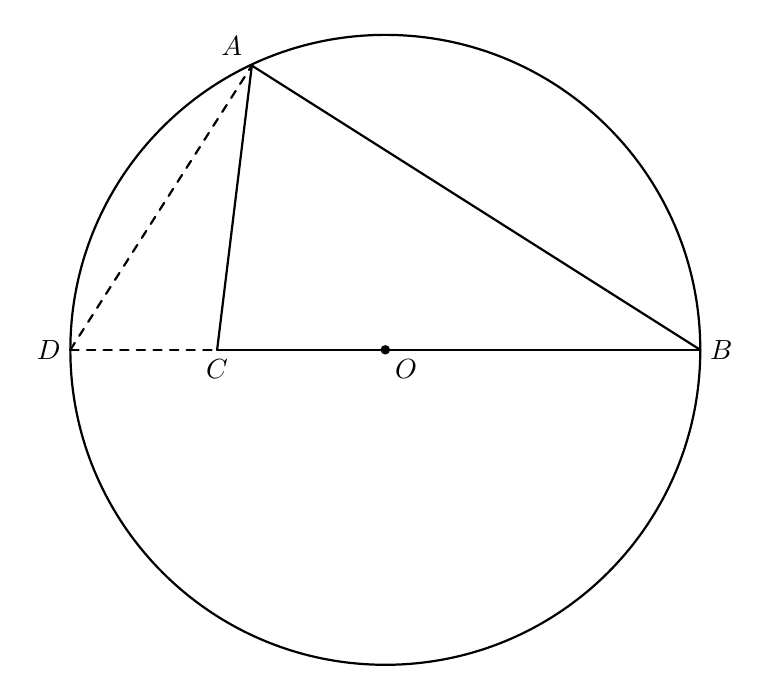
\begin{tikzpicture}[scale=1, line cap=round, line join=round]
  \coordinate (O) at (0,0);
  \coordinate (A) at (-1.695,3.61);
  \coordinate (B) at (4,0);
  \coordinate (C) at (-2.136,0);
  \coordinate (D) at (-4,0);

  \draw[thick] (O) circle (4);
  \draw[thick] (A) -- (C);
  \draw[thick] (A) -- (B);
  \draw[thick] (C) -- (B);
  \draw[thick,dashed] (D) -- (A);
  \draw[thick,dashed] (D) -- (C);
  \draw[fill=black] (O) circle (1.5pt);

  \node[above left] at (A) {$A$};
  \node[right] at (B) {$B$};
  \node[below] at (C) {$C$};
  \node[left] at (D) {$D$};
  \node[below right] at (O) {$O$};
\end{tikzpicture}
\end{document}
